\subsection{Quản lý ảnh}

Sau khi đăng nhập thành công, hệ thống sẽ điều hướng người dùng đến trang chủ thư viện ảnh, nơi người dùng có thể xem các ảnh đã tải lên theo ngày / tháng / năm. Ngoài ra người dùng có thể bấm vào từng ảnh để xem thông tin ảnh. tại đây người dùng có thể thực hiện các chức năng như xóa ảnh, yêu thích ảnh, đổi tên ảnh và xem thông tin chi tiết của ảnh như thời gian chụp, vị trí chụp, các tag liên quan đến ảnh và các khuôn mặt được nhận diện trong ảnh như hình \ref{fig:gallery}.

\begin{figure}[H]
    \centering
    \begin{subfigure}{0.32\textwidth}
        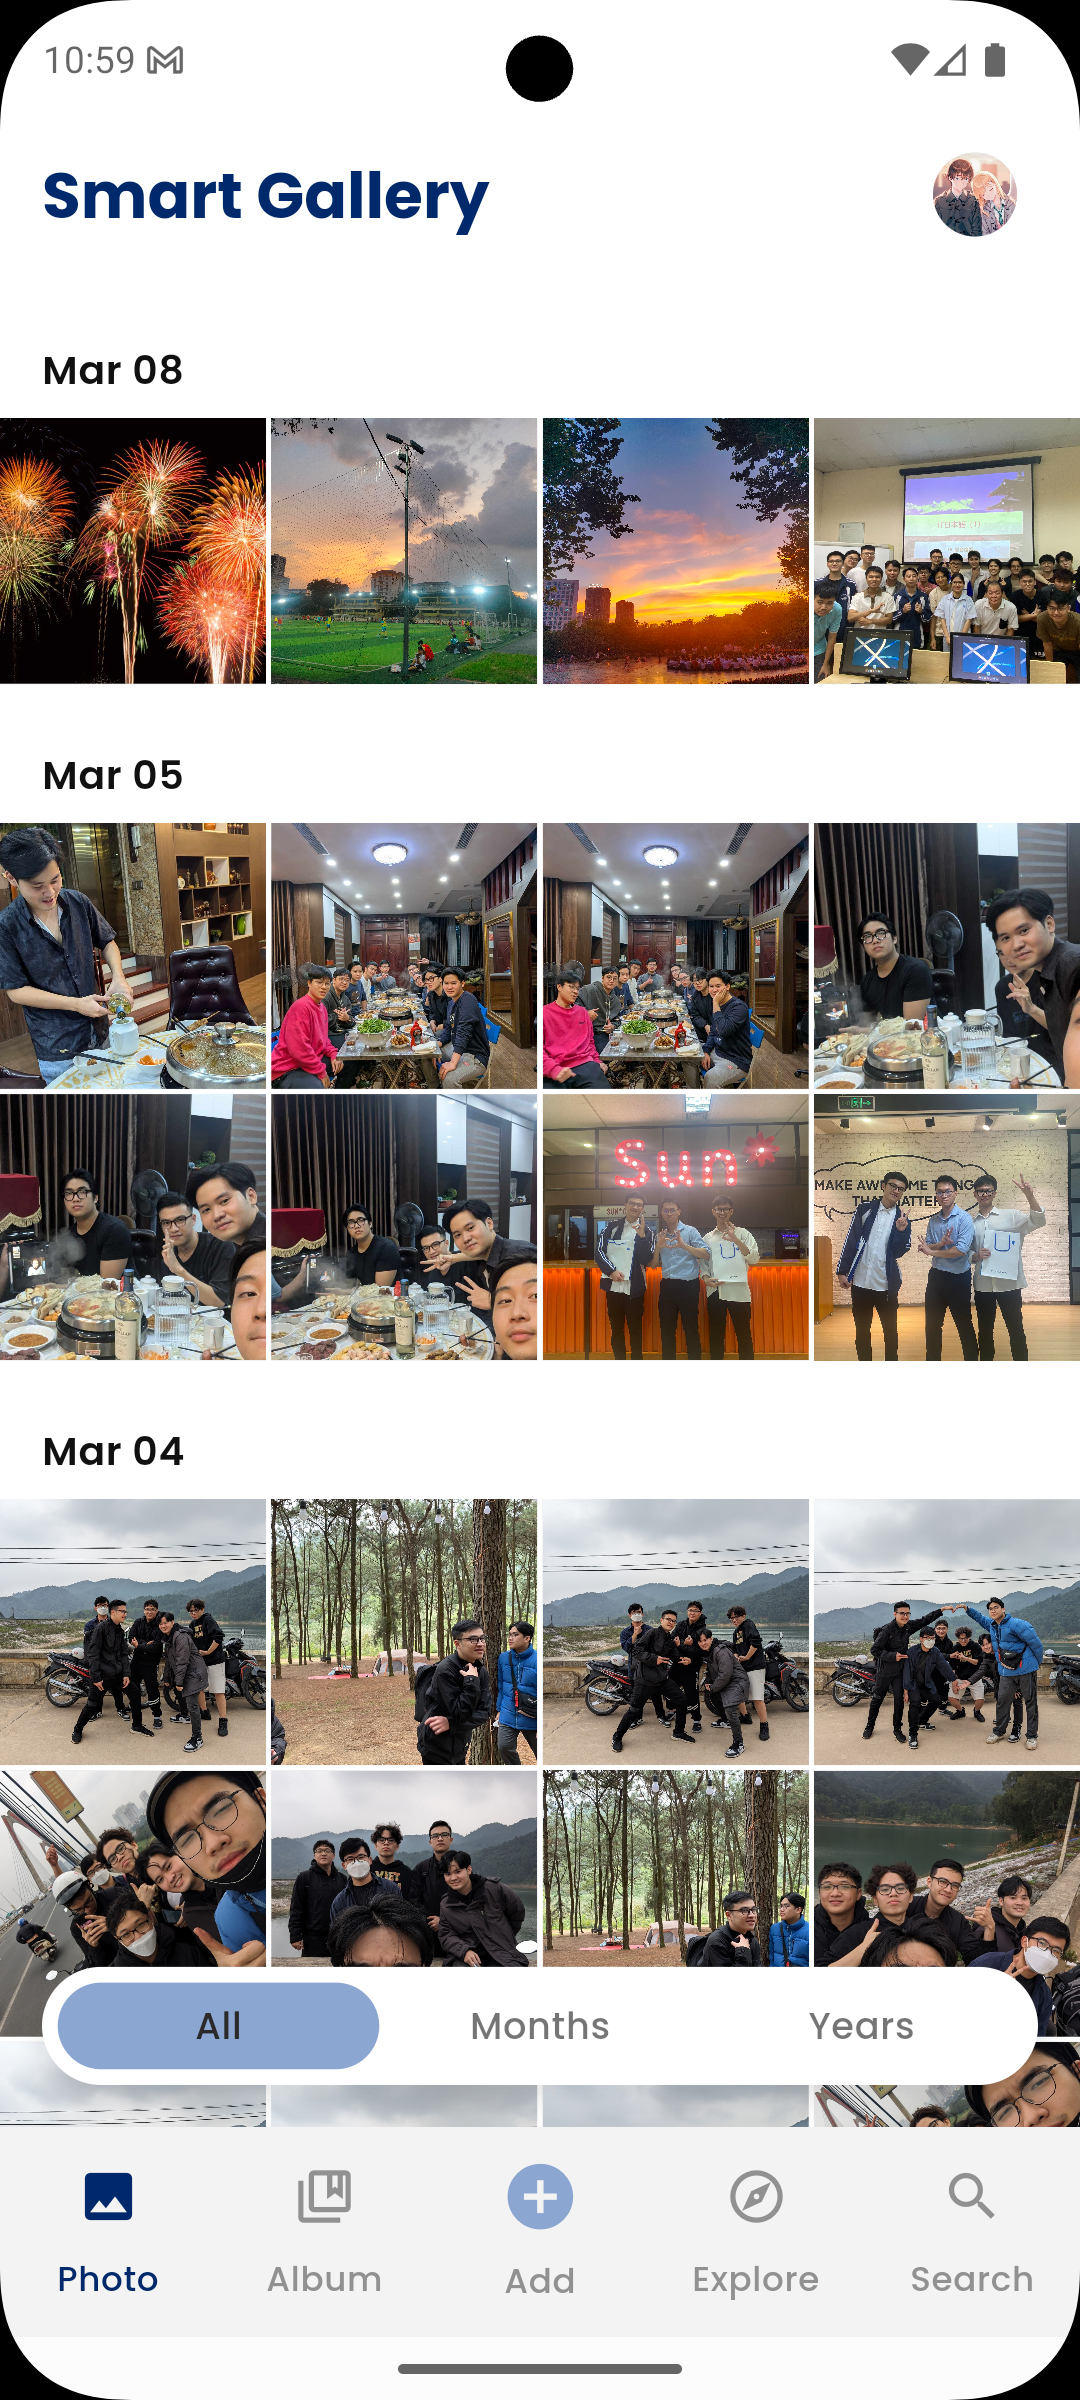
\includegraphics[width=1\linewidth]{figures/c4/4-2/gallery_1.png} 
        \caption{Xem ảnh theo ngày}
    \end{subfigure}
    \hfill
    \begin{subfigure}{0.32\textwidth}
        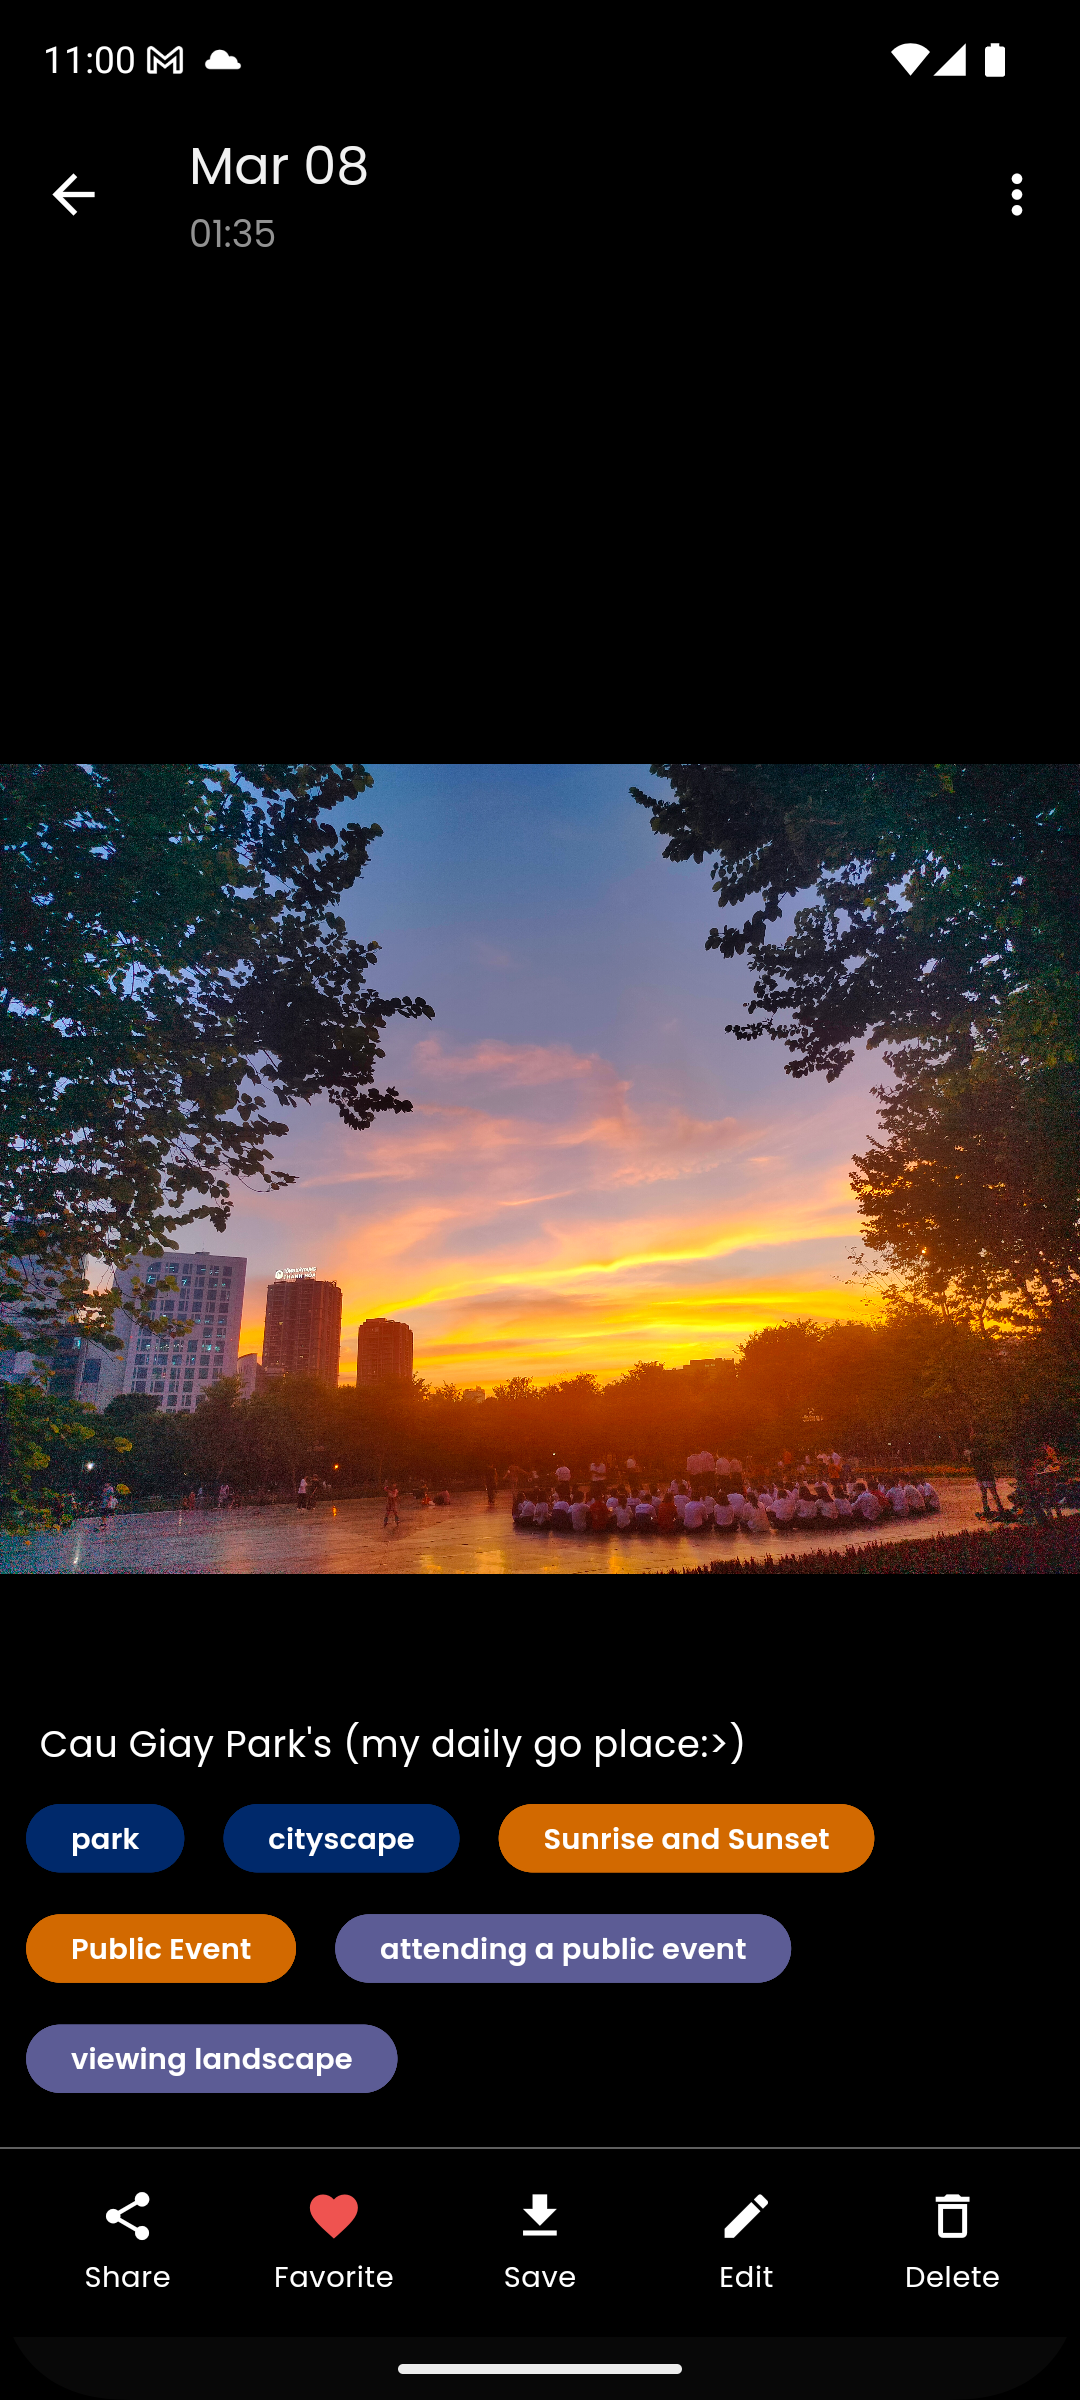
\includegraphics[width=1\linewidth]{figures/c4/4-2/image.png} 
        \caption{Xem ảnh}
    \end{subfigure}
    \hfill
    \begin{subfigure}{0.32\textwidth}
        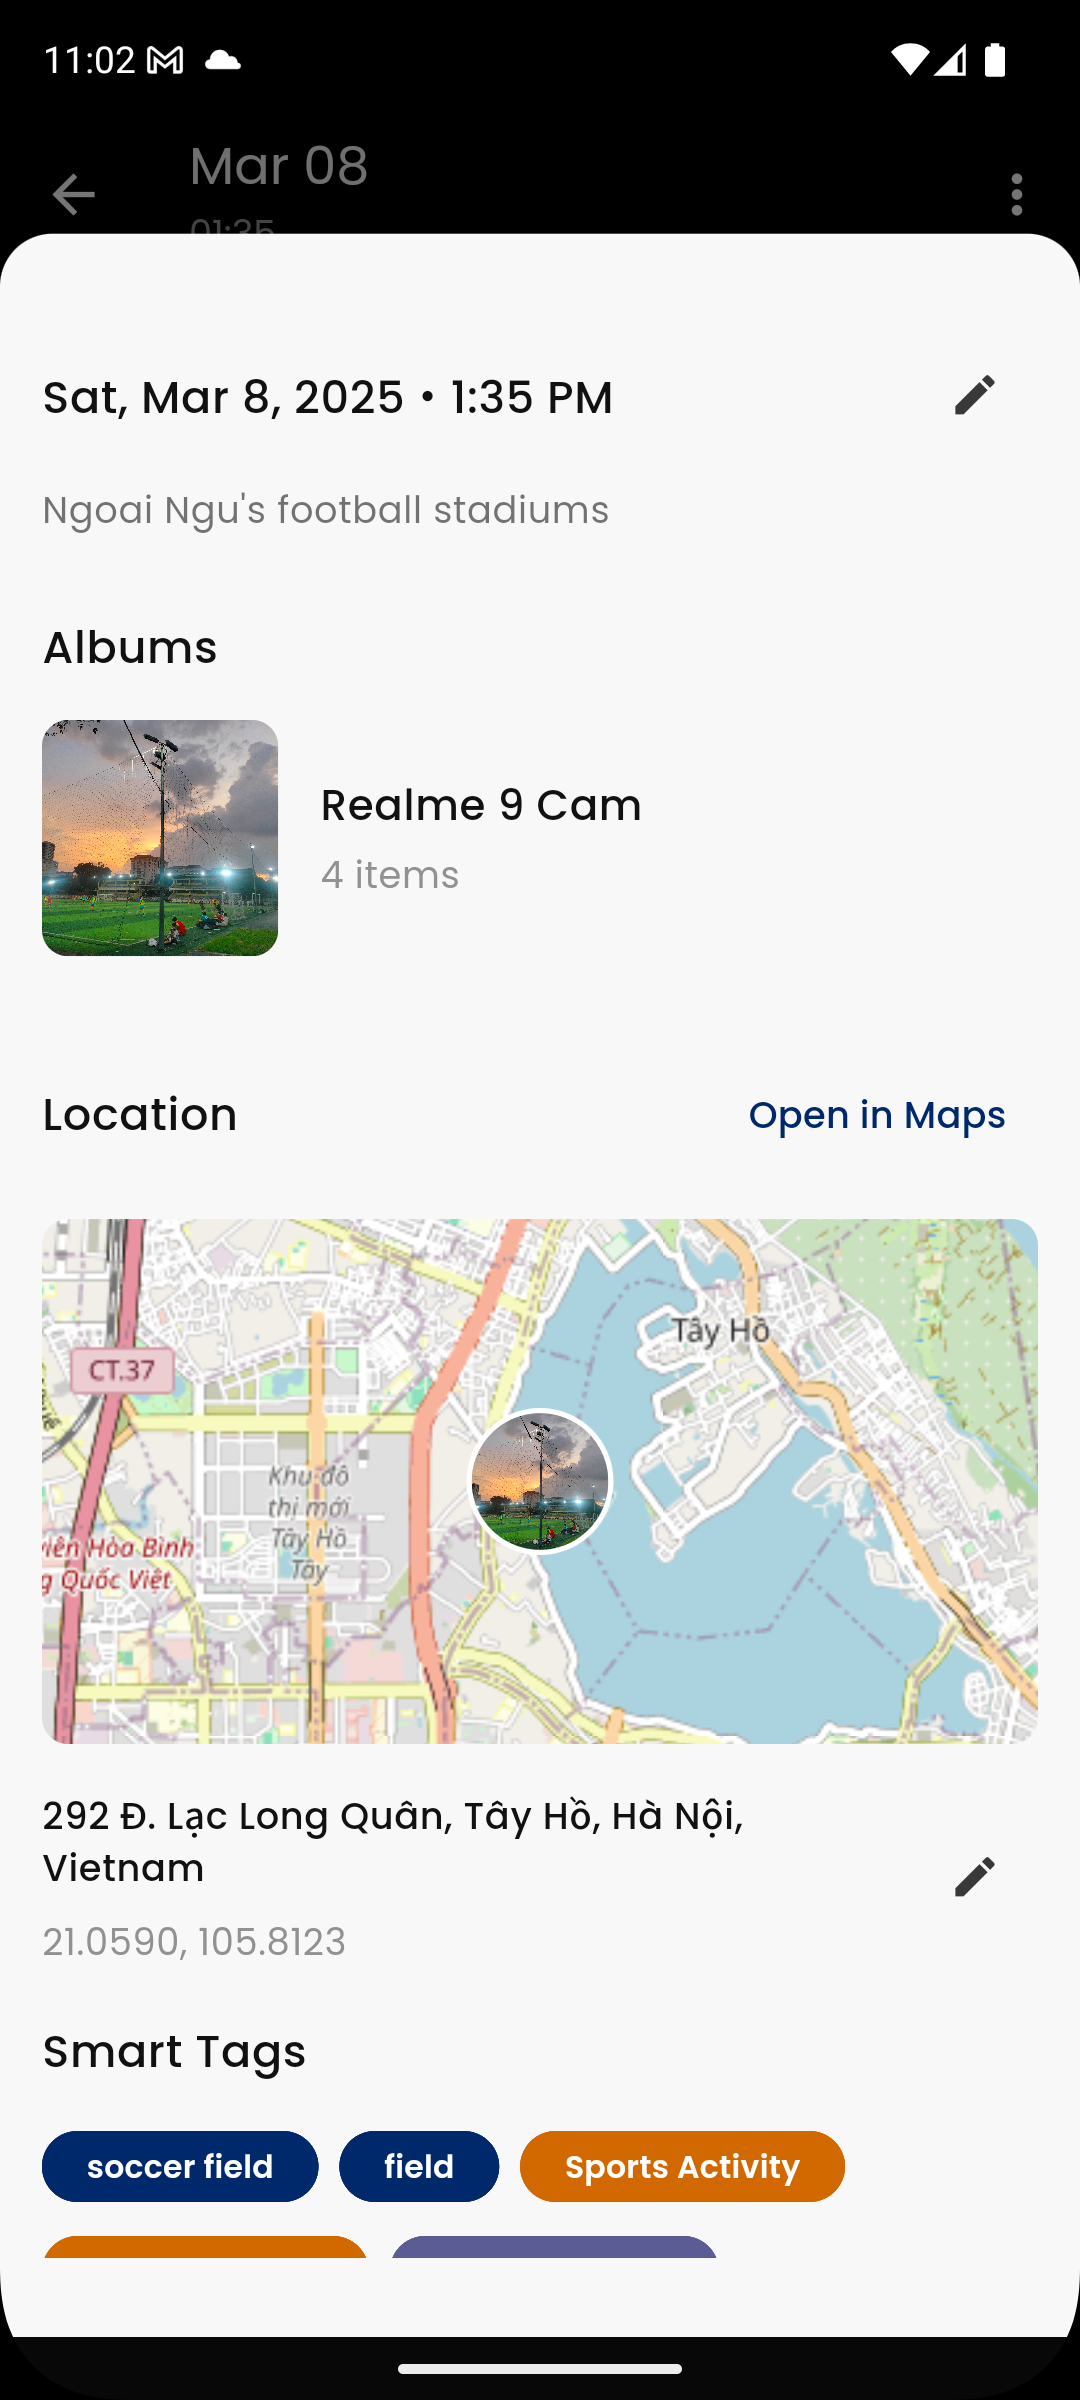
\includegraphics[width=1\linewidth]{figures/c4/4-2/image_info.png} 
        \caption{Xem thông tin }
    \end{subfigure}
    \caption{Giao diện thư viện ảnh.}
    \label{fig:gallery}
\end{figure}

% \begin{figure}[H]
%     \centering
%     \begin{subfigure}{0.48\textwidth}
%         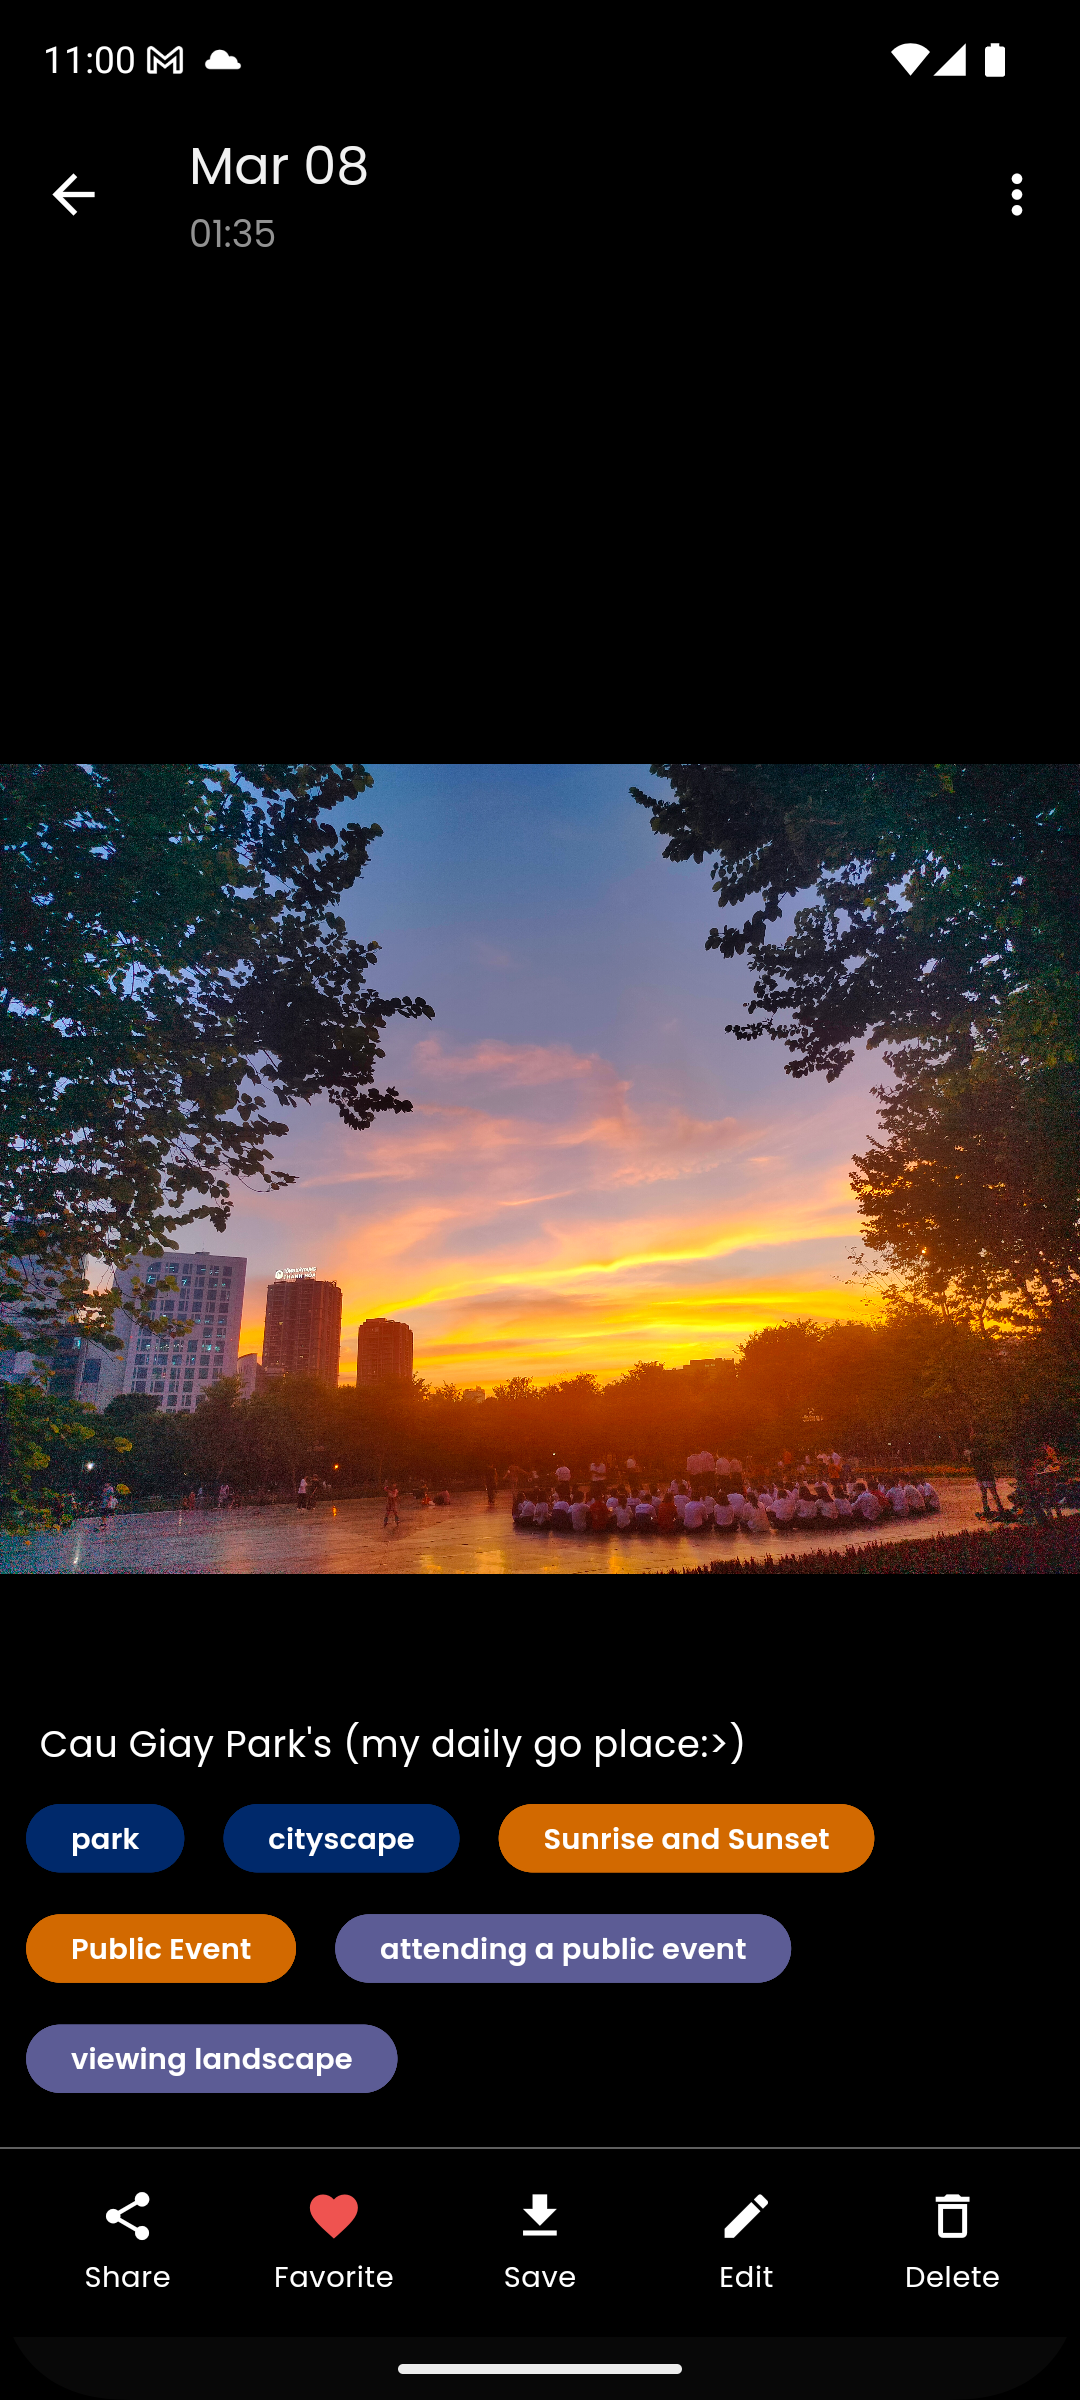
\includegraphics[width=1\linewidth]{figures/c4/4-2/image.png} 
%         \caption{Xem ảnh}
%     \end{subfigure}
%     \hfill
%     \begin{subfigure}{0.48\textwidth}
%         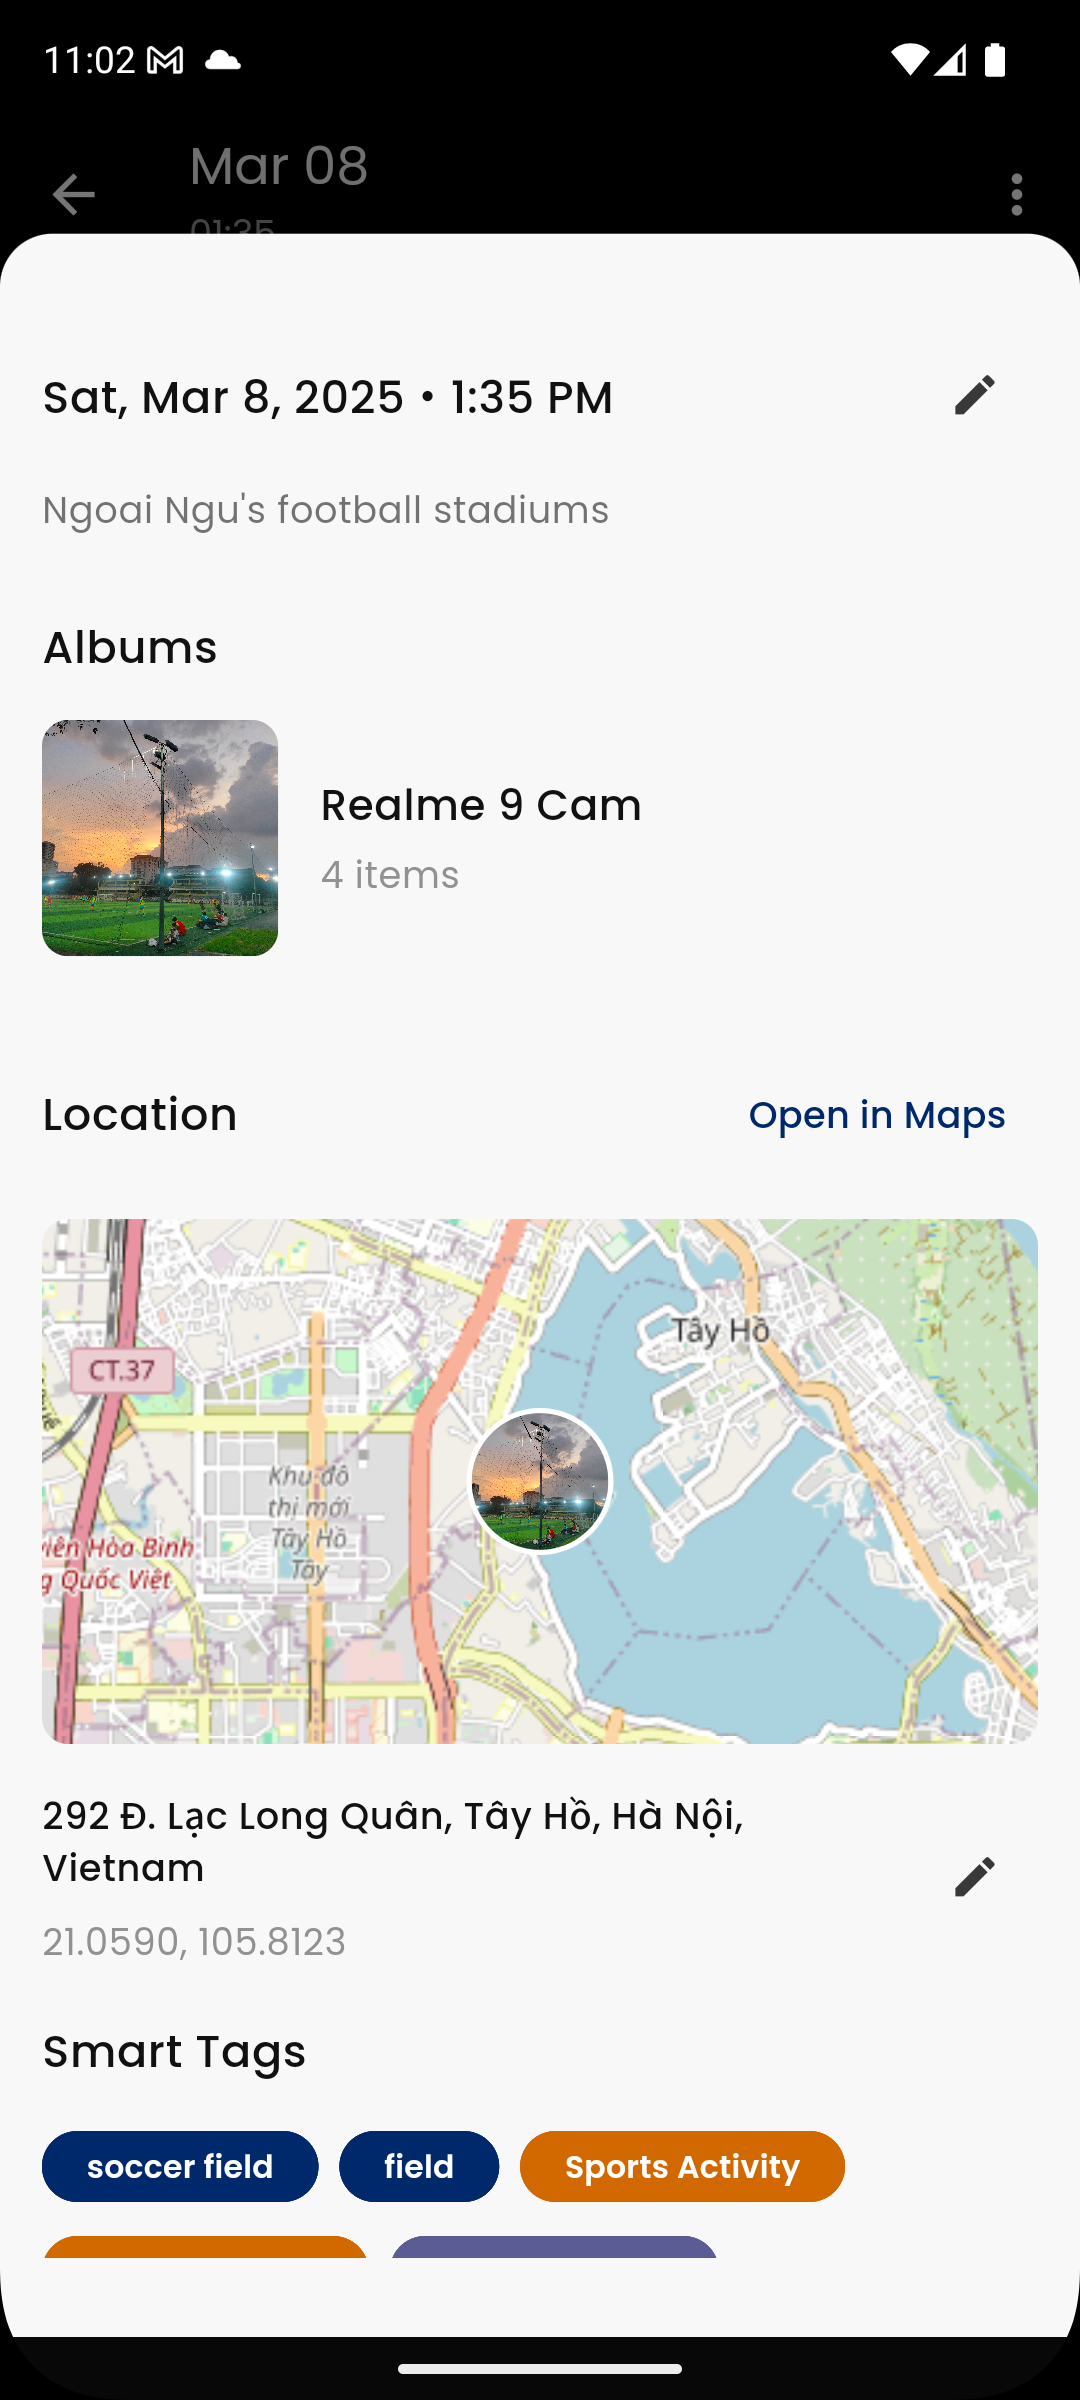
\includegraphics[width=1\linewidth]{figures/c4/4-2/image_info.png} 
%         \caption{Xem thông tin }
%     \end{subfigure}
%     \caption{Giao diện thư viện ảnh.}
%     \label{fig:photo-info}
% \end{figure}